\ProvidesFile{chapters/ch-Event_Reconstruction.tex}

\chapter{Particle-Flow Event Reconstruction}
The CMS detector consists of several sub-detector layers that exploit the different properties of particles to identify them and measure their energy-momenta and trajectories.
For reconstructing particle object from their interaction with the detector, the CMS experiment has a developed a holistic particle-flow (PF) reconstruction algorithm that combines the measurements from all relevant sub-detector layers~\cite{Sirunyan:2270046}.
The algorithm links the charged-particle tracks measured in the inner silicon tracker with the energy deposits in the calorimeters and the muon tracks measured in the outer muon tracking system.
As there are trade-offs between reconstruction efficiency and misidentification rate, the criteria for classifying reconstructed objects are determined by dedicated CMS Physics Object Groups (POG) which perform expert analyses to optimize the efficiency and purity of object identification.

\section{Track and Vertex Reconstruction}
Track reconstruction is the determination of final state particles trajectories using the ionization trails left behind in the tracker sub-dectector layers, and is crucial for the identification and momenta measurement of charged particles.
Pile-up (PU) refers to the situation where multiple $pp$ collisions (vertices) occur within the same bunch crossing, and vertexing is the determination from which vertex in the bunch crossing the final state particles originated.
The primary vertex (PV) of an event is assumed to be the vertex corresponding to the hard-scatter interaction in the collision and is identified as the vertex with the highest sum of squared transverse momenta of its associated tracks.
Vertexing is also important for the identification of secondary vertices, i.e. vertices separated from the beam line by $\gtrapprox \SI{1}{\mm}$ or more, which are usually attributed to the decay of short-lived heavy flavor mesons.
Typical PU in CMS recorded data from 2016 through 2018 was around 20-30 vertices per bunch crossing, but high (low) extremes routinely occurred during the beginning (end) of beam fills due to instantaneous 
luminosity decay.
In the PF algorithm, iterative Kalman filtering (KF) is used to reconstruct the tracks and vertices of charged particles~\cite{Sirunyan:2270046}.
KF assumes that the residuals between the predicted and measured trajectories are Gaussian distributions.
The algorithm is seeded with tracks generated from two hits in consecutive layers in the pixel detector.
The KF fits the expected trajectory of the particles based on measured charge and momentum, accounts for multiple scattering and energy loss of particles in the detector material, and updates the track parameters based on measurements in each detector layer.
A visualization of the reconstructed tracks and identified vertices for an event with high PU recorded by the CMS detector in 2016 is shown in figure~\ref{Pileup}.
\begin{figure}[!h]
  \begin{center}
    \begin{tabular}{c}
        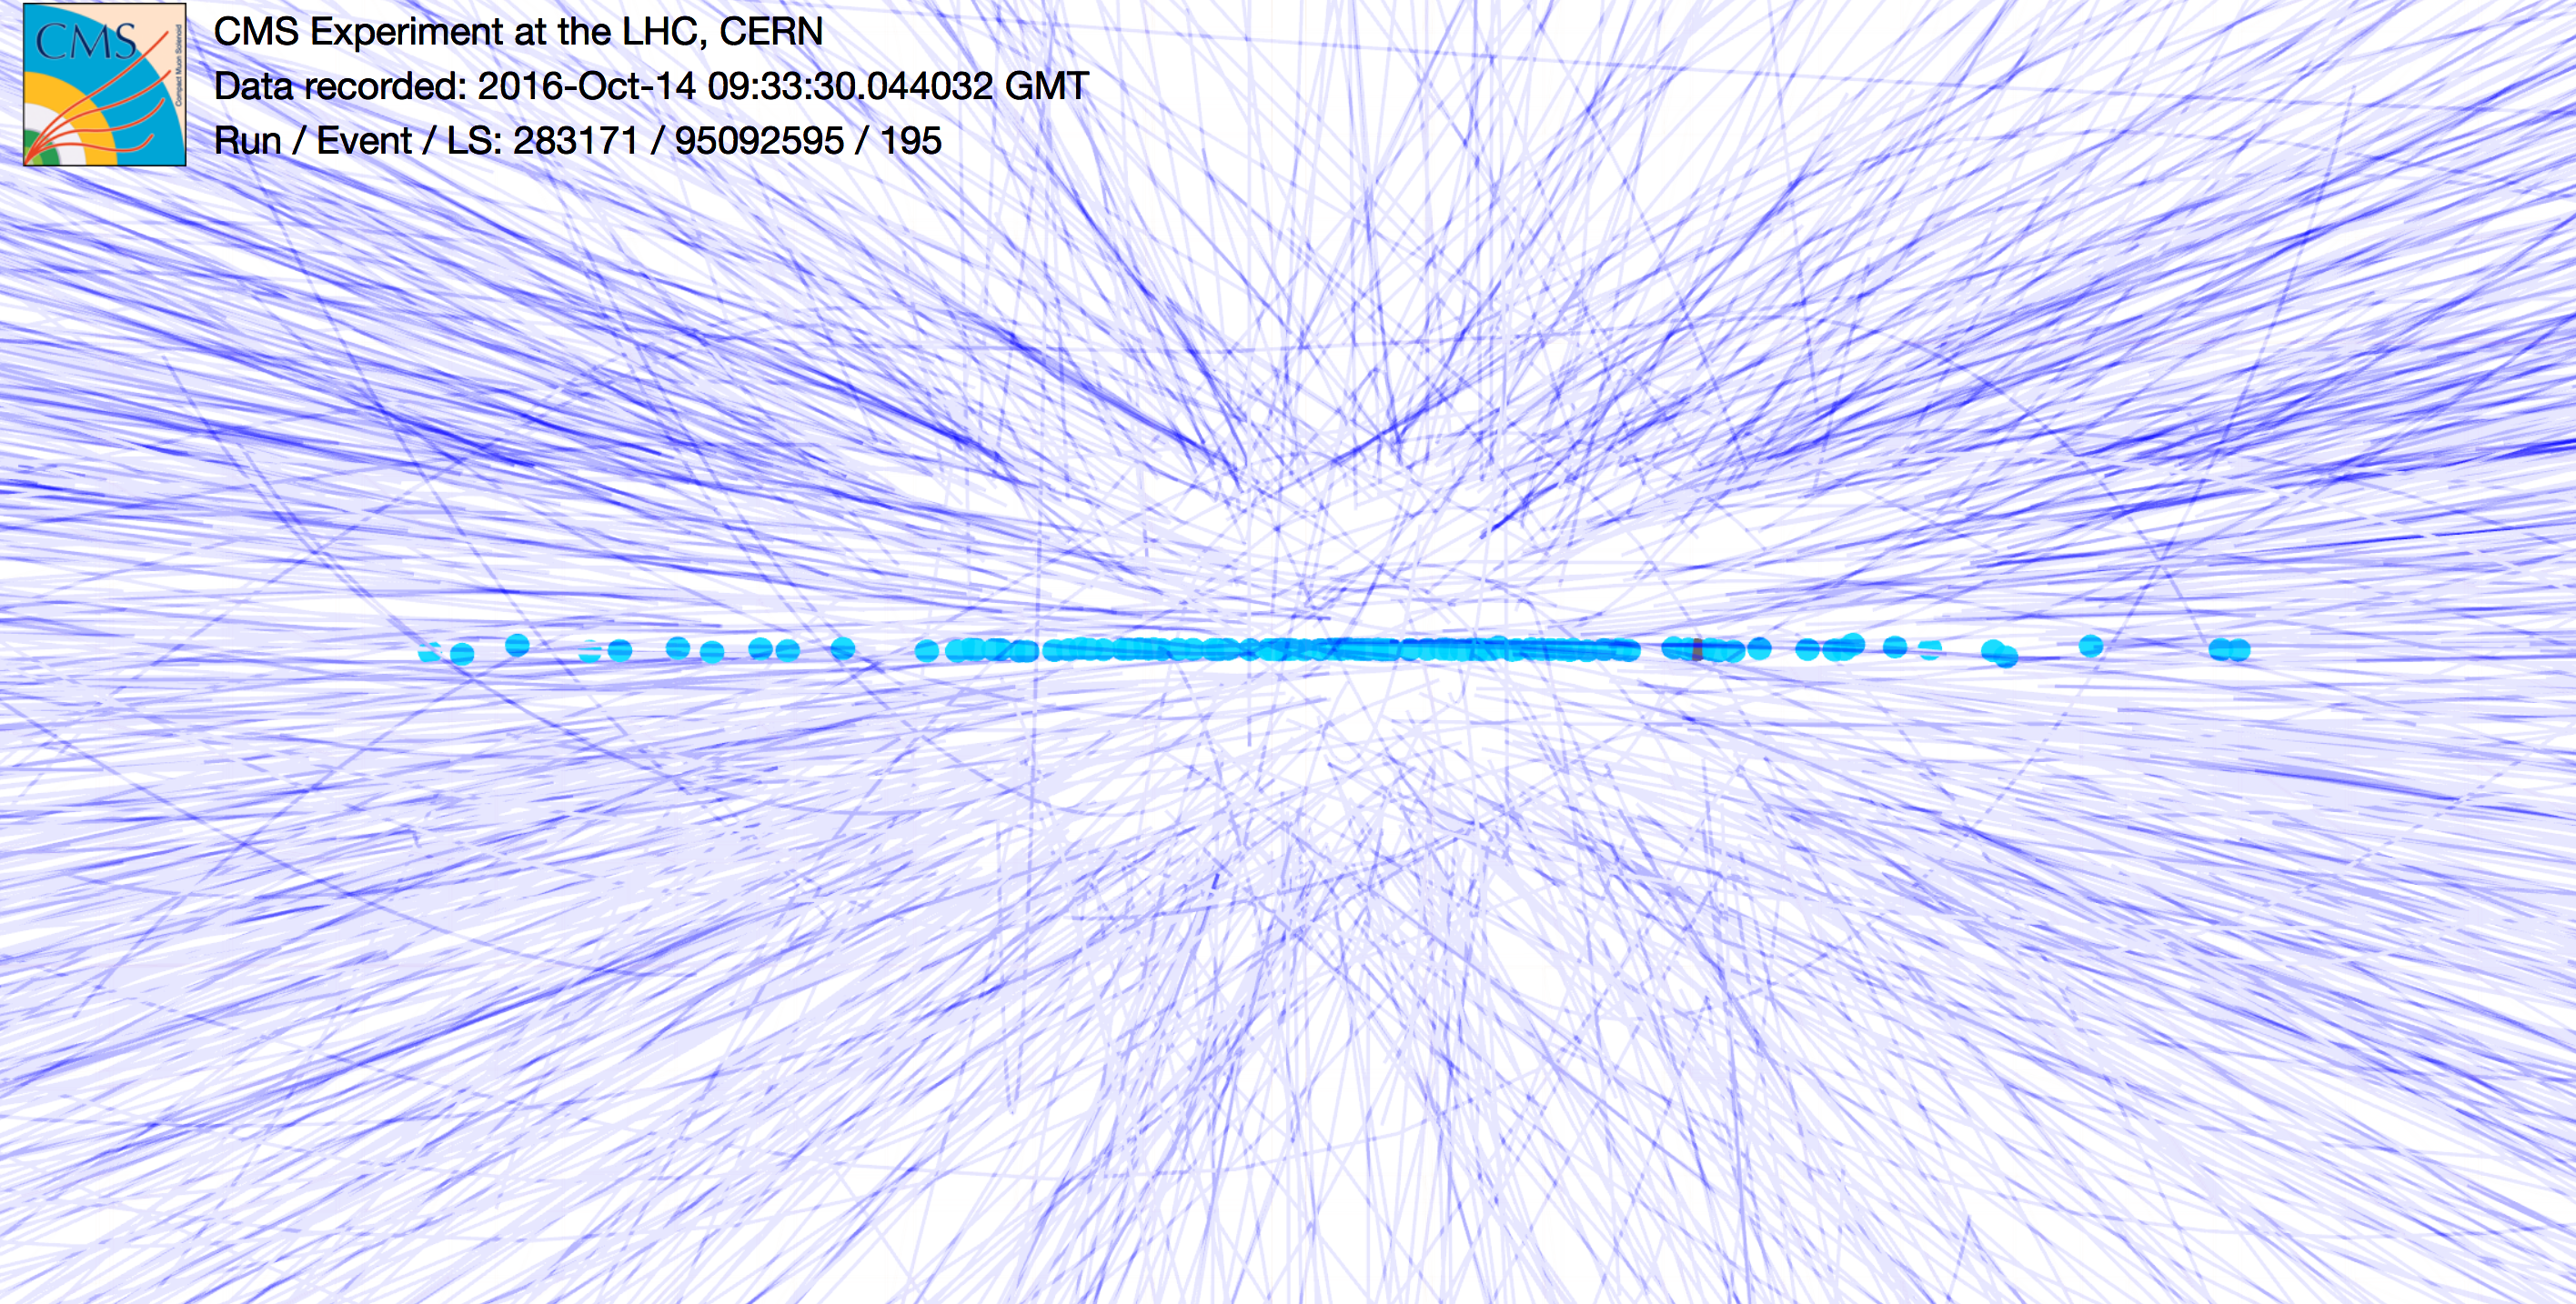
\includegraphics[width=0.6\textwidth]{fig_Event_Reconstruction/Pileup.png}
    \end{tabular}
    \caption{A visualization of the reconstructed tracks and identified vertices for an event with high PU recorded by the CMS detector in 2016~\cite{Collaboration:2231915}.
            }
    \label{Pileup}
  \end{center}
\end{figure}

\section{Object Reconstruction}
The main particles that are directly detected by CMS are muons, electrons, photons, charged hadrons (e.g. protons, pions, kaons), and neutral hadrons (e.g. neutrons).
An illustration of the signatures left behind by these particles in the various sub-detectors is shown in figure~\ref{CMS_Layers}.
\begin{figure}[!h]
  \begin{center}
    \begin{tabular}{c}
        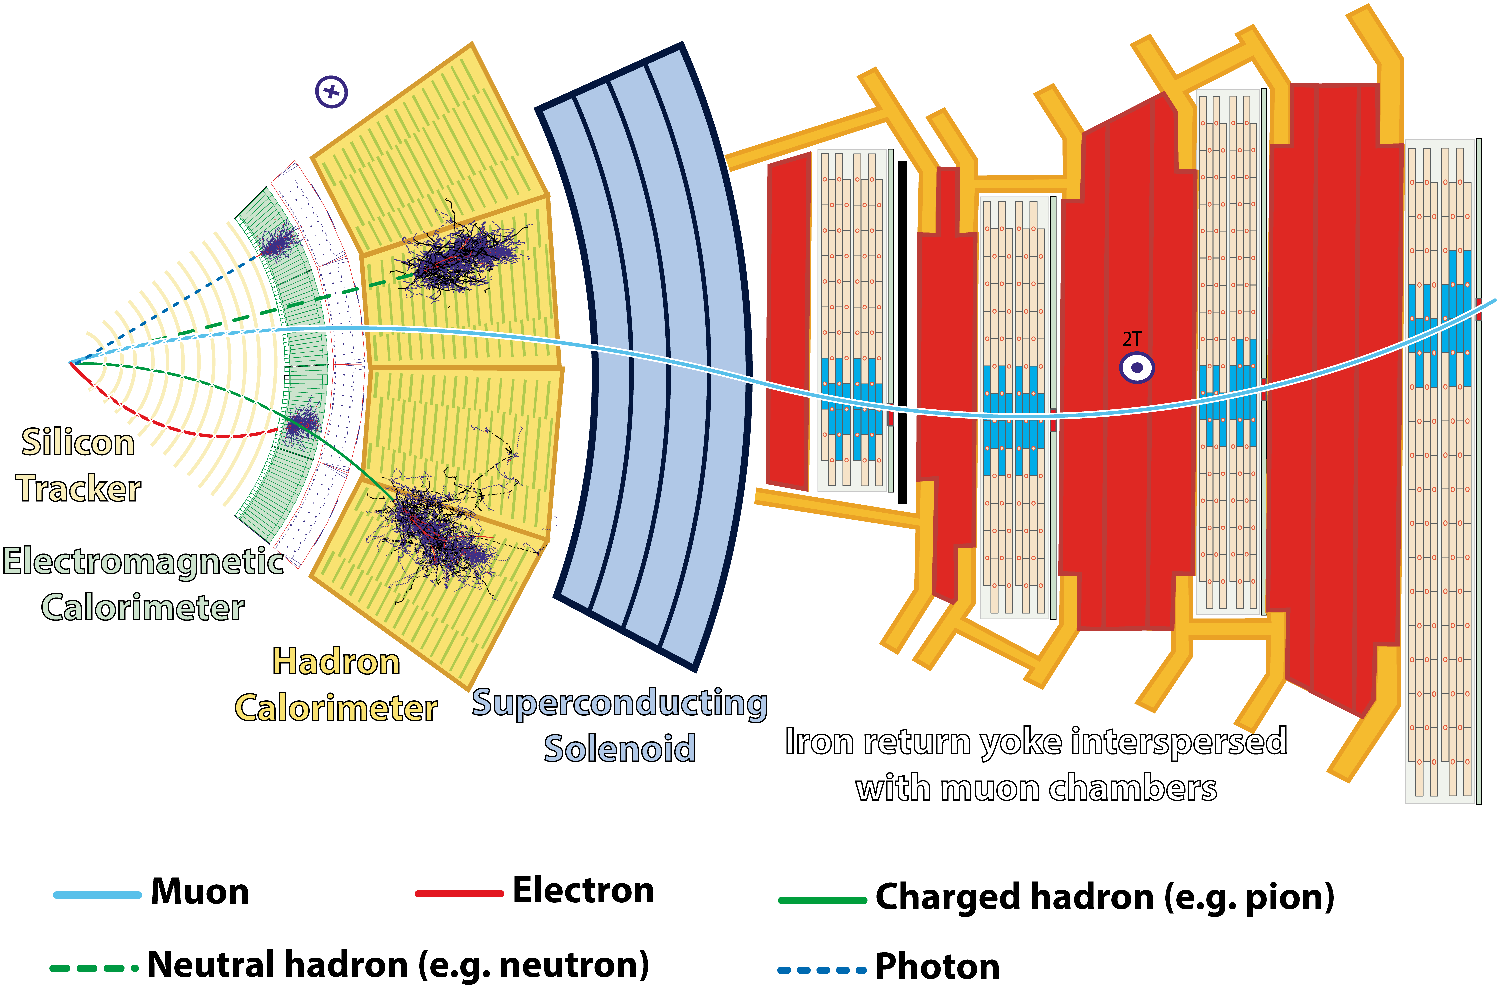
\includegraphics[width=0.9\textwidth]{fig_LHC_CMS/CMS_Layers.png}
    \end{tabular}
    \caption{Muons, electrons, photons, charged hadrons, and neutral hadrons are directly detected by CMS and are identified by the signatures they leave behind in the various sub-detectors~\cite{Sirunyan:2270046}.
            }
    \label{CMS_Layers}
  \end{center}
\end{figure}
The PF algorithm identification and reconstruction sequence first identifies and reconstructs muon candidates, then electron and photon candidates, and finally charged and neutral hadron candidates.
After each step, tracks and clusters of reconstructed objects are removed from further consideration for subsequent steps.
Photon reconstruction was not used for the measurement presented in this paper, and therefore is skipped in the following subsections.

\subsection{Muons}
Muons leave tracks in the silicon tracker, their trajectories are curved due to the presence of the magnetic field of the solenoid, and they penetrate through the calorimeters and solenoid to leave ionization trails in the outer tracker.
As is implied by its name, the CMS experiment was designed to detect muons with high reconstruction efficiency and low misidentification rate.
Muons that are reconstructed independently in both the inner tracking detector and the outer muon system are referred to as global muons.
A global fit of the muon momentum using both sub-detectors has momentum resolution of $1-3\%$ for low momentum muons ($\SI{20}{\GeV} < \pT < \SI{200}{\GeV}$), depending on $\eta$, and $5\%$ for high momentum muons ($\sim \SI{1}{\TeV}$)~\cite{Chatrchyan:1129810}.
If hadron shower remnants "punch-through" the HCAL and solenoid into the outer muon system, they may be misreconstructed as muons, but additional criteria can be used to balance the efficiency and purity of muon identification.

\subsection{Electrons}
Electrons leave ionization trails in the silicon tracker, their trajectories are curved due to the presence of the magnetic field of the solenoid, and their energy is deposited in the ECAL.
Electron tracks are seeded from the ECAL clusters and extrapolated back to the inner silicon tracker.
Gaussian Sum Filtering (GSF), which assumes that the residuals between the predicted and measured trajectories are sums of multiple Gaussian distributions, is used to reconstruct electrons.
Due to the total radiation length of the inner silicon tracker, the probability that an electron emits a bremsstrahlung photon by interacting with tracker material is about $85\%$~\cite{Sirunyan:2270046}.
Thus the ECAL clusters from the electron and the bremsstrahlung photons in a window around the electron direction are grouped into a "supercluster."
For non-isolated electrons, such as those produced in jets, the superclustering can result in large inefficiencies, so the ECAL seeding criteria is restricted with isolation requirements.

\subsection{Jets}
Quarks and gluons produced in $pp$ collisions hadronize into collimated showers of particles called jets.
Jets primarily consist of hadrons, but also can contain photons and leptons when hadrons in the jet radiate or decay before reaching the detector.
Charged hadrons leave tracks in the silicon tracker, their trajectories are curved due to the presence of the magnetic field of the solenoid, deposit some energy in the ECAL, and exhaust their energy in the HCAL, while neutral hadrons do not leave tracks in the silicon tracker and exhaust their energy in the HCAL.
The granularity of the inner silicon tracker is sufficiently fine to provide separation of individual particle trajectories within jets, and energy clusters are deposited in the calorimeters from the particles in the shower.
The anti-$k_T$ jet clustering algorithm groups reconstructed particles into jets by merging the pair of particles with the smallest distance, calculating new distances between the merged object and the remaining particles, and repeating this process until all particles have been merged into jet objects~\cite{Matteo_Cacciari_2008}.
For anti-$k_T$ jet clustering, the distance $d_{ij}$ between two particles $i$ and $j$ is defined as:
\begin{align}
d_{ij} = min(\sfrac{1}{p_{T,i}^2}, \sfrac{1}{p_{T,j}^2}) \times \sfrac{{\Delta R_ij}^2}{R^2}
\end{align}
where $\Delta R$ is the angular separation between objects, defined in equation~\ref{DeltaR}, and $R$ is the radius parameter that determines the size of individual jets.
The PF algorithm reduces the amount of energy that is mistakenly assigned to a jet due to pileup by removing clusters attributed to tracks originating at pileup vertices.

\subsection{Missing Transverse Energy}
For collisions at the LHC, there is no net momentum or force in the transverse direction, so \pT is conserved and sums to zero for both incoming protons and outgoing particles after the collision.
This property is useful for inferring the production of particles invisible to the detector, i.e. neutrinos, from the missing transverse energy (MET):
\begin{align}
\vec{E}_T^{miss}=-\sum_{i} \vec{p}_{T,i}
\end{align}
the negative vector sum of the transverse momenta for all PF reconstructed particles in an event~\ref{met_schematic}.
\begin{figure}[!h]
  \begin{center}
    \begin{tabular}{c}
        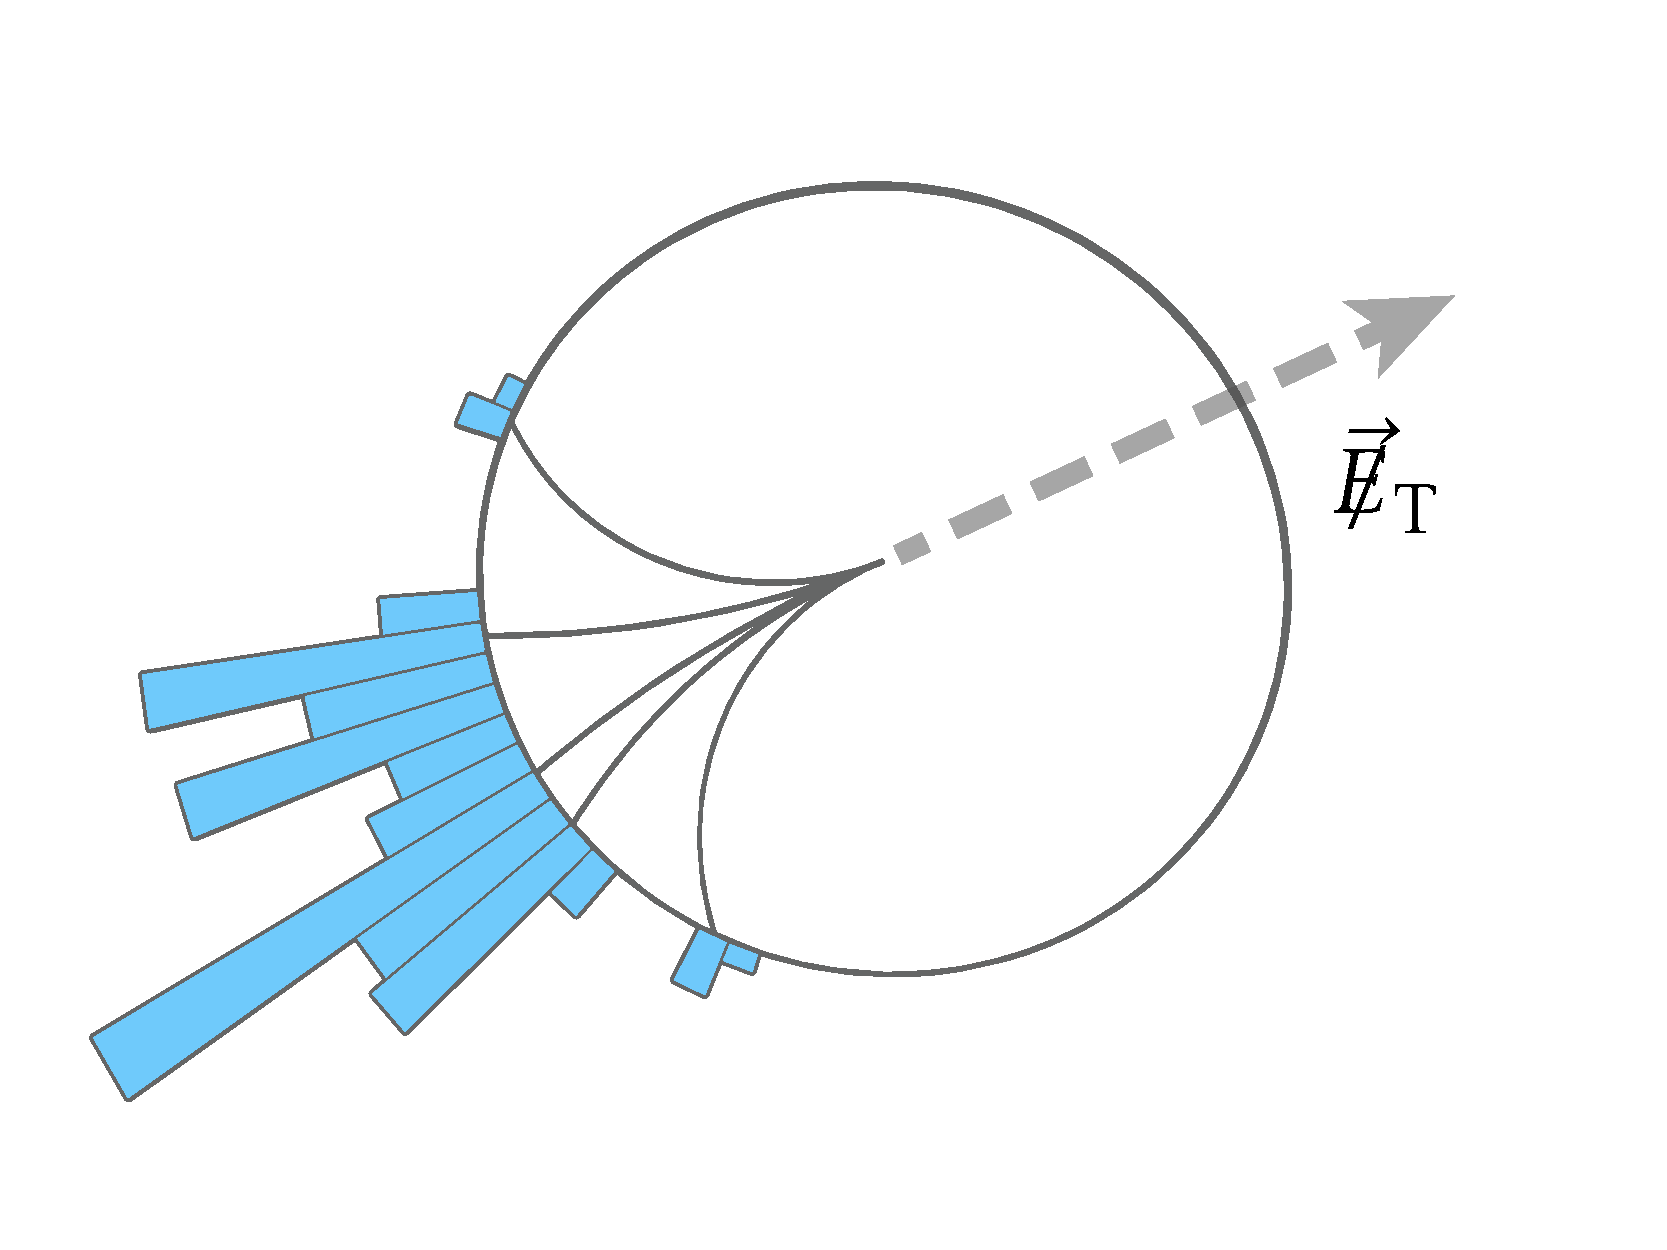
\includegraphics[width=0.3\textwidth]{fig_Event_Reconstruction/met_schematic.pdf}.
    \end{tabular}
    \caption{Schematic diagram for \MET, the negative vector sum of the transverse momenta for all reconstructed particles in an event~\cite{METSchematicDiagram}.
            }
    \label{met_schematic}
  \end{center}
\end{figure}


